% !TeX encoding = UTF-8
% !TeX program = lualatex
% !TeX spellcheck = en_US
% !TeX root = thesis.tex

\chapter{Case study - BRAC University}
\label{chap:case_study_BRAC_U}
\index{BRAC}


\blindtext[2]



\begin{figure}[hbt]
	\centering
	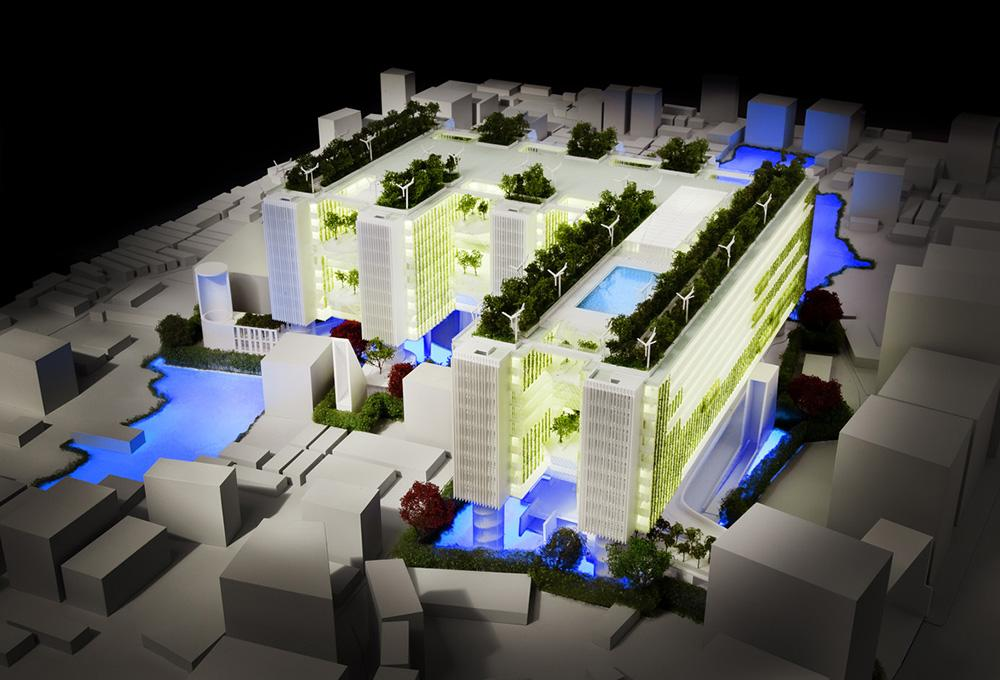
\includegraphics[width=0.9\linewidth]{images/BRAC_Model}
	\caption[BRAC University]{BRAC University \citep{WOHA}.}
	\label{fig:bracmodel}
\end{figure}





\clearpage

\thispagestyle{empty}
\vspace*{\fill}
\begin{center}
\sffamily This page is intentionally left blank
\end{center}
\vspace*{\fill}


\clearpage

%\newpage
\paragraph{Reference layout}

To start with, the results of the reference layout V1-4w will be discussed with regard to conventional visualization techniques.
%In this section, the simulation results for BRAC University regarding \ACR s and CO$_2$ concentration as well as age of air are going to be shown and discussed.
All following horizontal cross-sections are taken at (\SI{1.35}{\metre}) above the floor and clipped to the size depicted in the figures. It should  also be noted that the \ACR\ illustrations are not true to scale and solely serve the purpose of depicting the geometric features. For true scale geometries please refer to \fref{sec:appendix:BRAC_geometry}.

\Fref{fig:V1-4w_flow_field} illustrates the horizontal cross-section\footnote{Note that horizontal cross-sections of $|u|$ are instantaneous snapshots of the flow field. A visual examination against iteration-averaged values did not show different flow characteristics.} of V1-4w colored by $|u|$. This visualization is a conventional method of illustrating a flow field.
The flow is characterized by the following characteristics:

\begin{enumerate}[label=(\Alph*)]
	
	\item Flow separation with a reattachment point of approximately \SI{30}{m} into the building block.
	
	\item  Constriction of the flow in staircase area; following the continuity constraint,  the velocities increased by a factor of $\sim$\num{2}.
	
	\item Local velocity differences that create vortices in the windward \CR.
	
	\item  Indefinite flow structure in leeward \CR s where the ventilation pattern changes from a \CR\ of type (C) to (D).
	
\end{enumerate}





\begin{figure}[!hb]
	\centering
	\subfloat[][conventional flow field]{
	\begin{annotatedFigure}{
			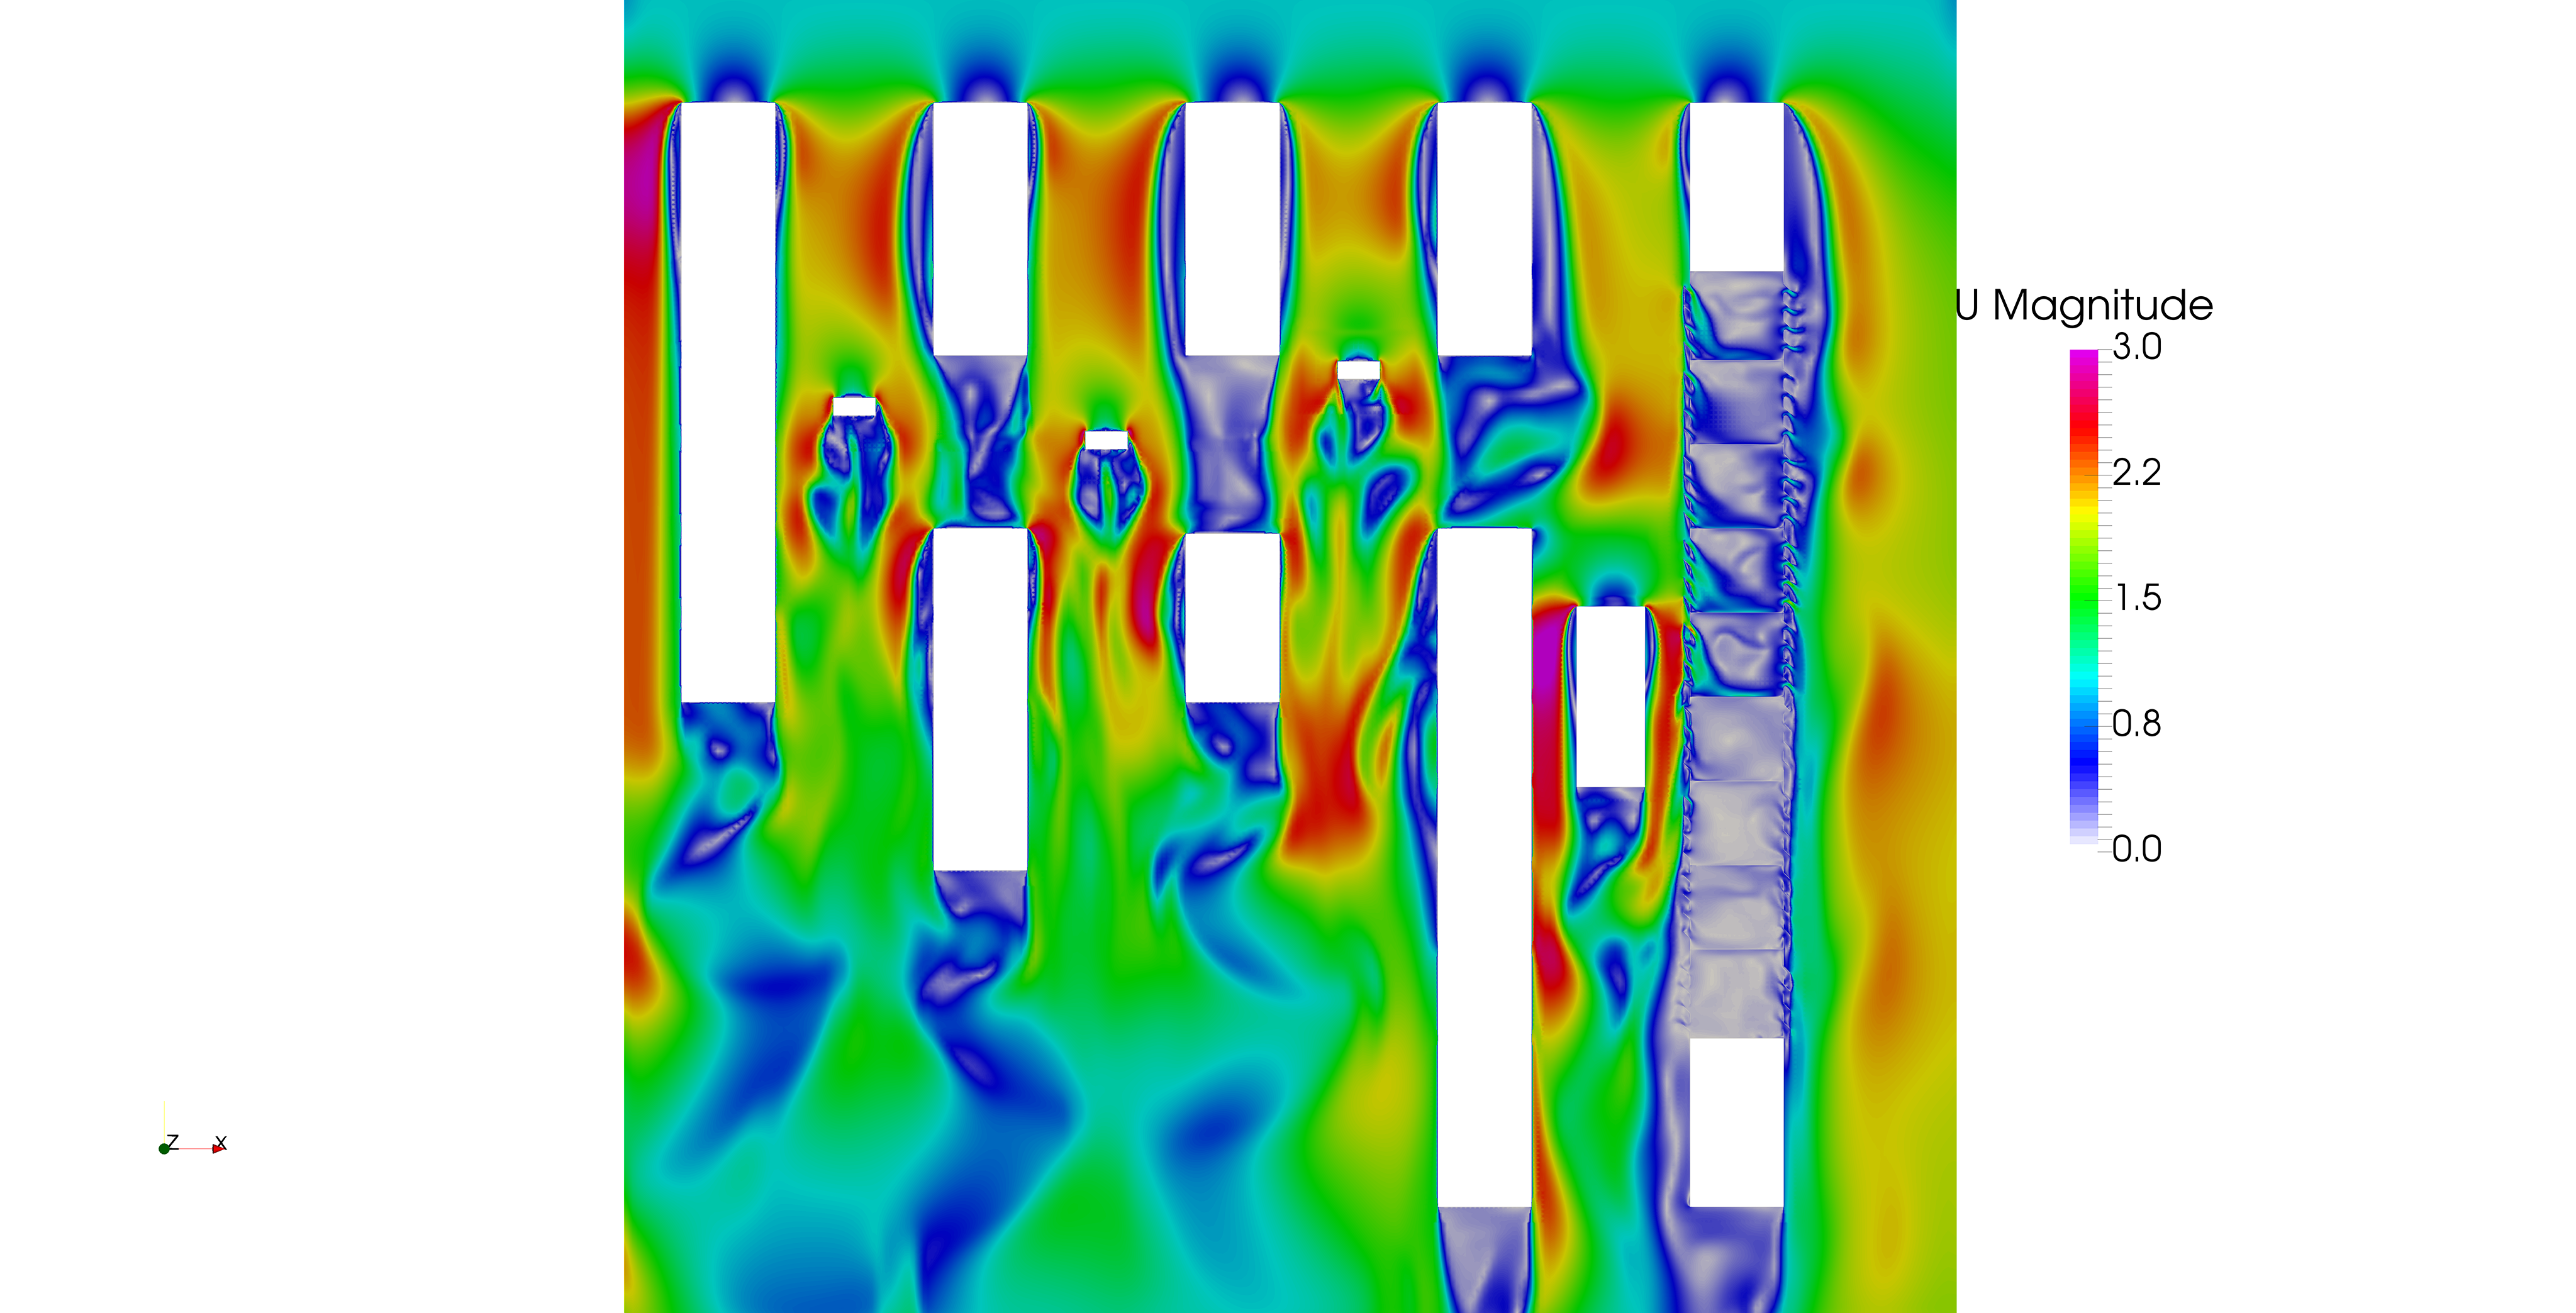
\includegraphics[width=0.35\linewidth, trim= 86cm 10cm 35cm 2.5cm, clip]{images/topview/V1-4w/topview_magU}}
		\annotatedFigureBox{0.2,0.85}{0.90,0.95}{A}{0.2,0.85} 	
		\annotatedFigureBox{0.02,0.27}{0.38,0.51}{B}{0.02,0.25} 
		\annotatedFigureBox{0.33,0.55}{0.63,0.65}{C}{0.33,0.55} 	
		\annotatedFigureBox{0.25,0.09}{0.63,0.25}{D}{0.25,0.09} 		
		%(links , unten)	(rechts, oben)
	\end{annotatedFigure} \hspace*{0.2cm}
	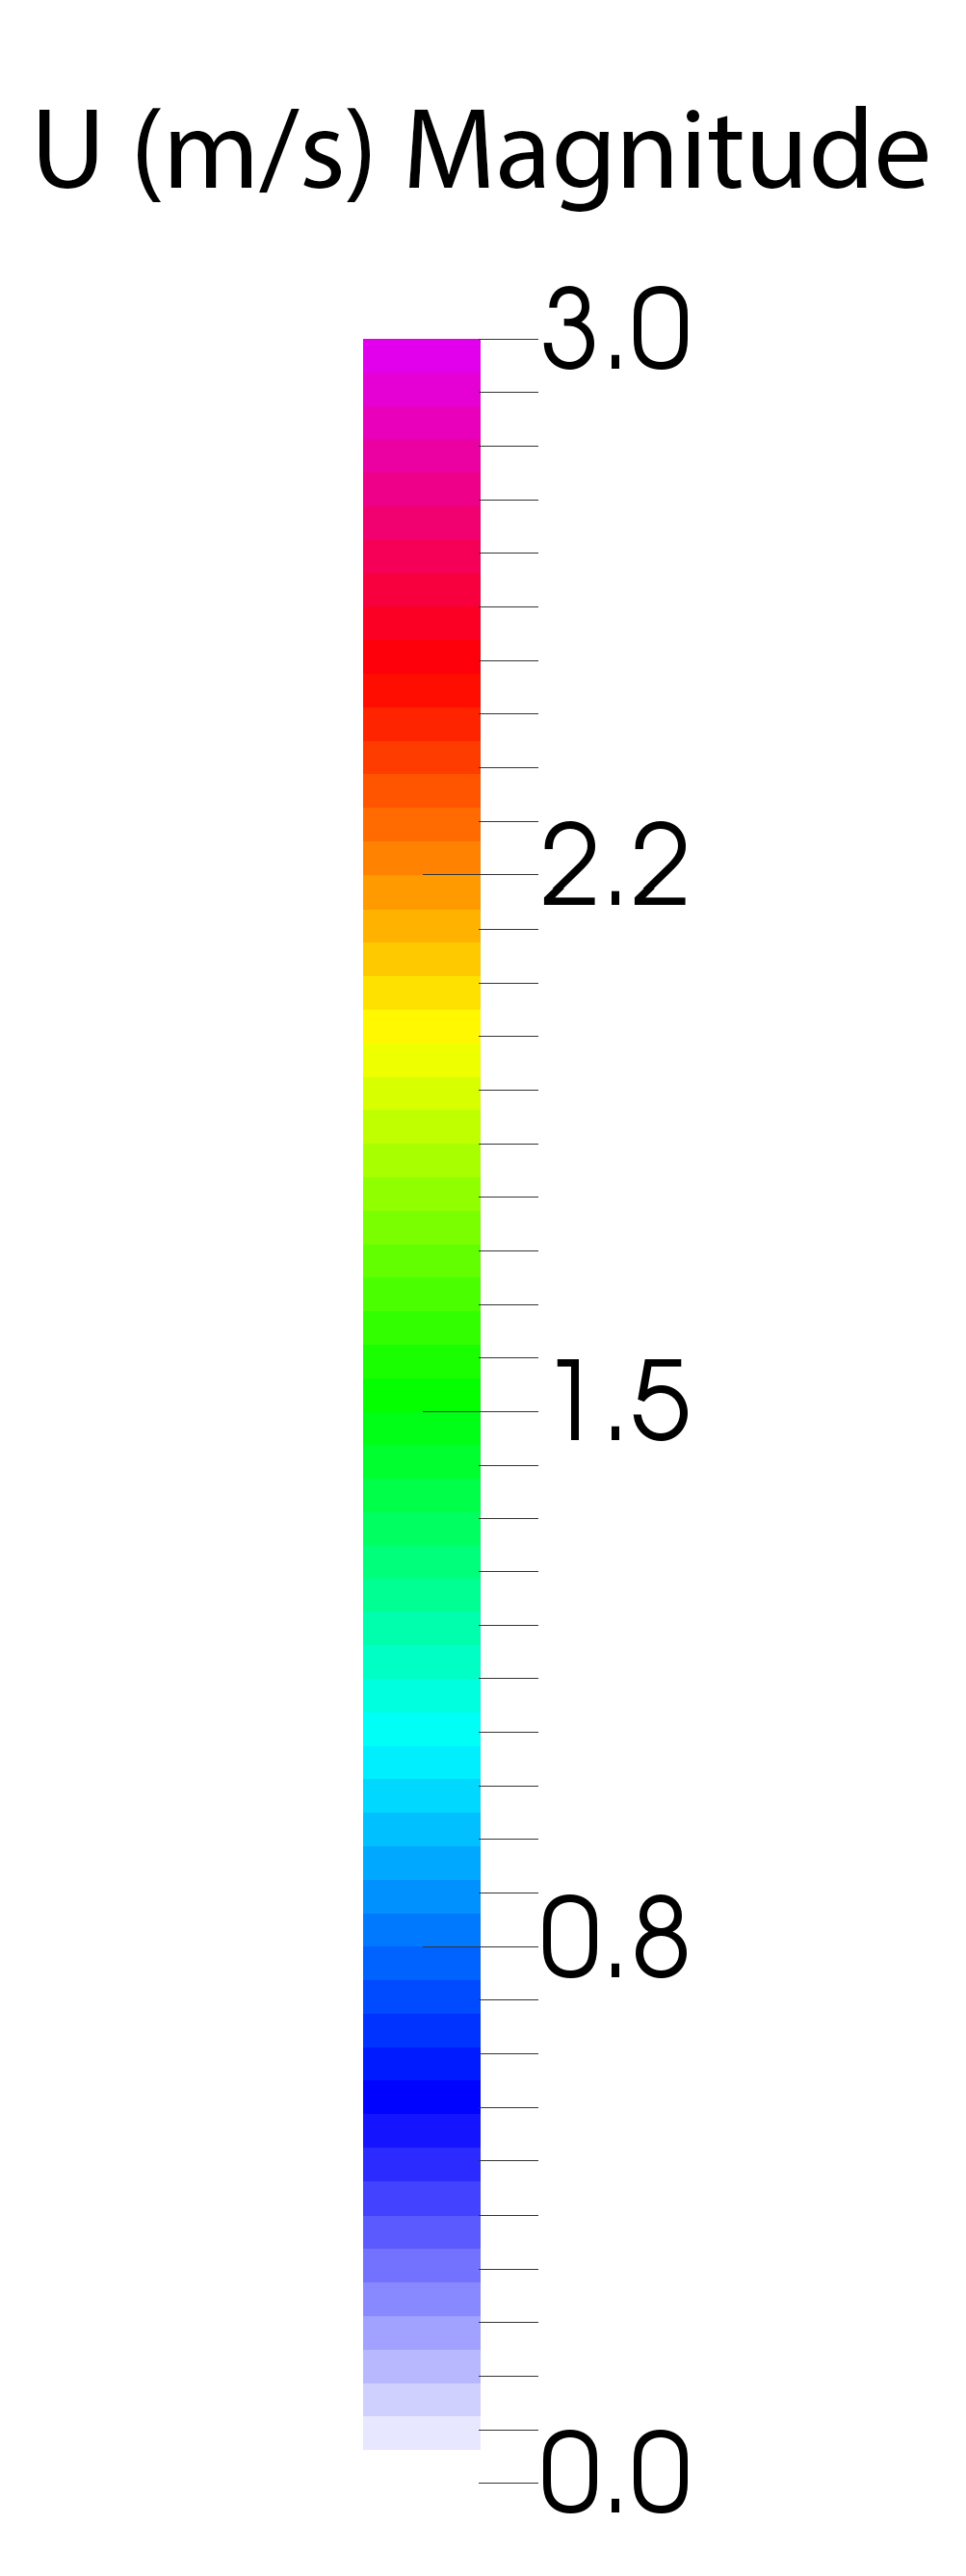
\includegraphics[width=0.25\linewidth, trim= -5cm -14cm 0cm 0cm, clip]{images/topview/scale_magU}}
	%	\hspace*{3cm}\llap{\raisebox{1cm}{%minus raisebox schibet nach unten
	%			%	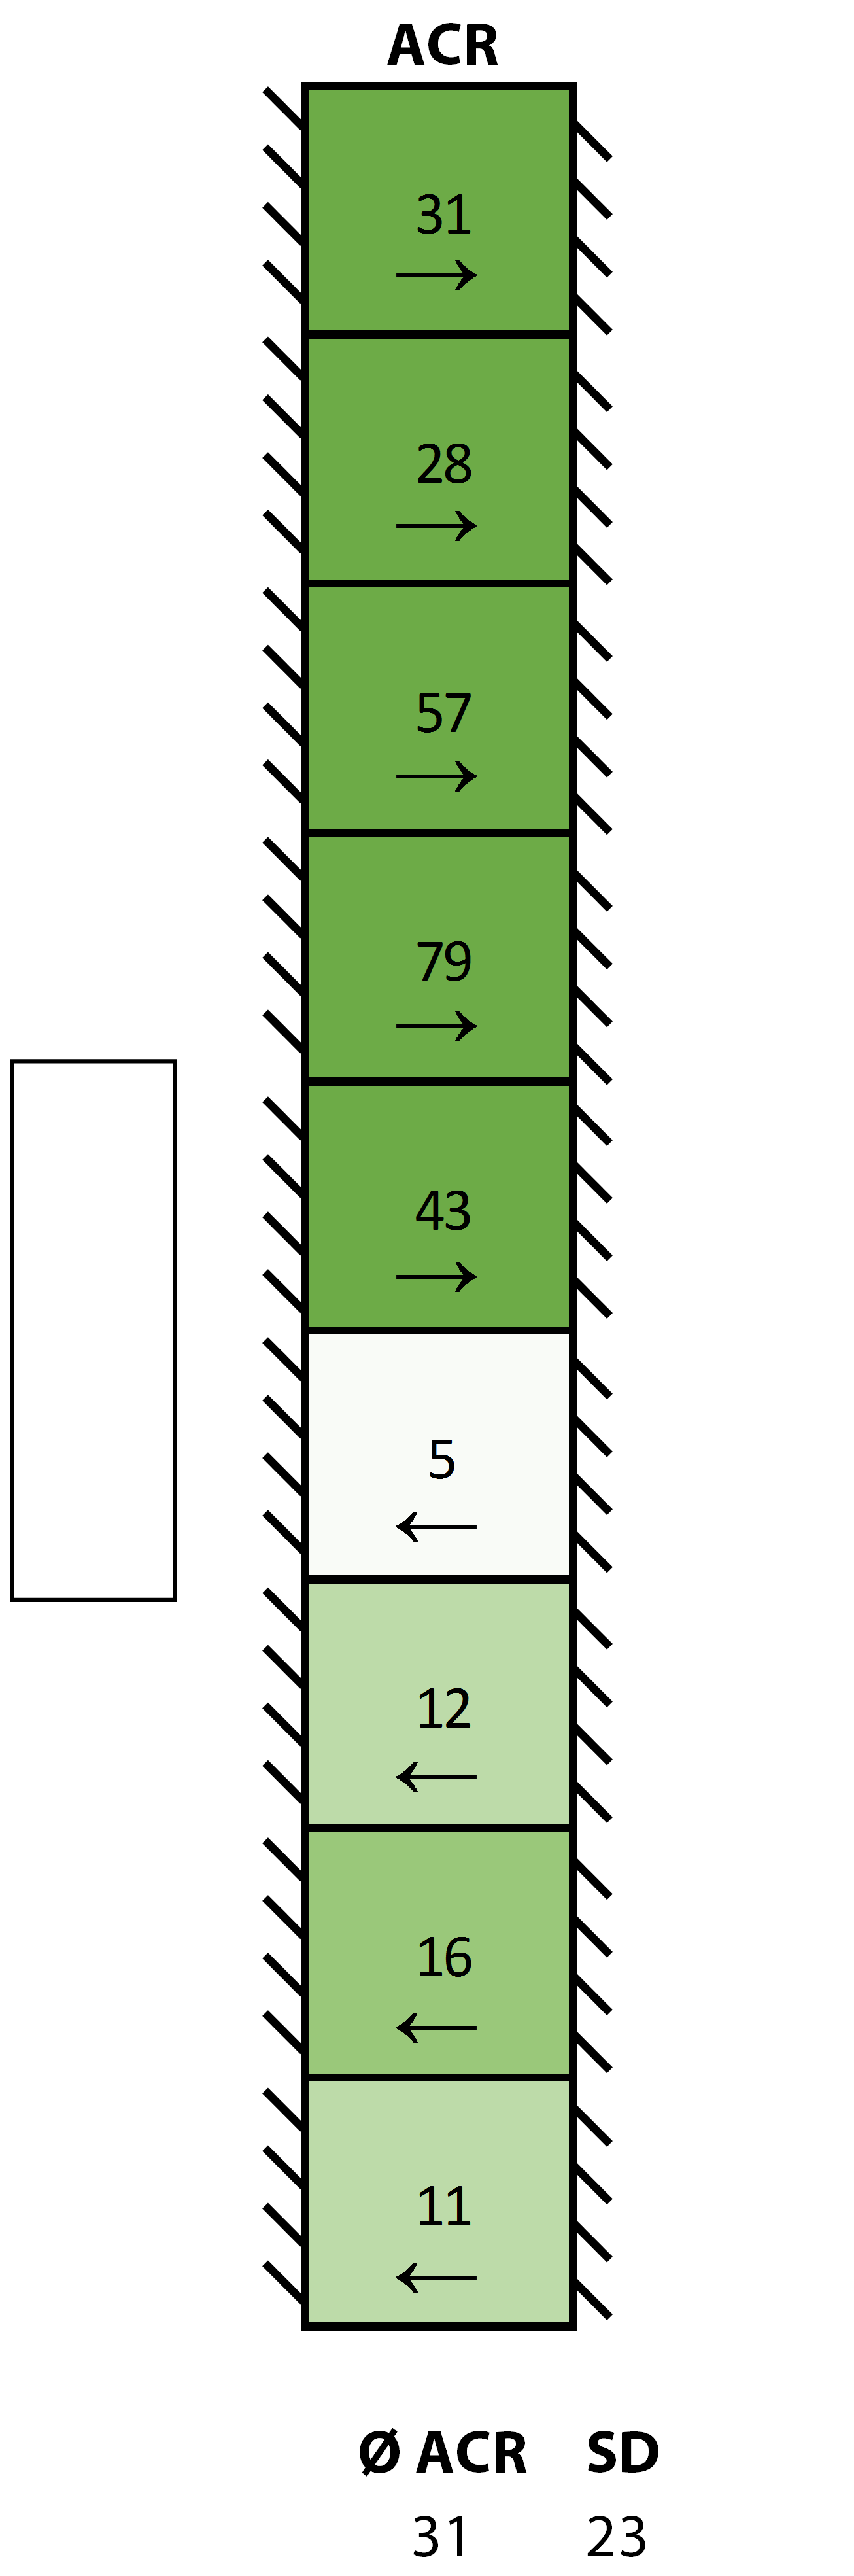
\includegraphics[width=0.14\linewidth, trim= 1.4cm 1cm 1.4cm 0.45cm, clip]{images/ACR/ACR_V1-4w}	
	%	}}
	\begin{tikzpicture}[remember picture, overlay]
	\node[yshift=8cm] {
\includegraphics[scale=0.3, trim= 0cm 0cm 0cm -2cm, clip]{images/arrow_N}};
	\end{tikzpicture}
	\subfloat[][ACRs]{	
	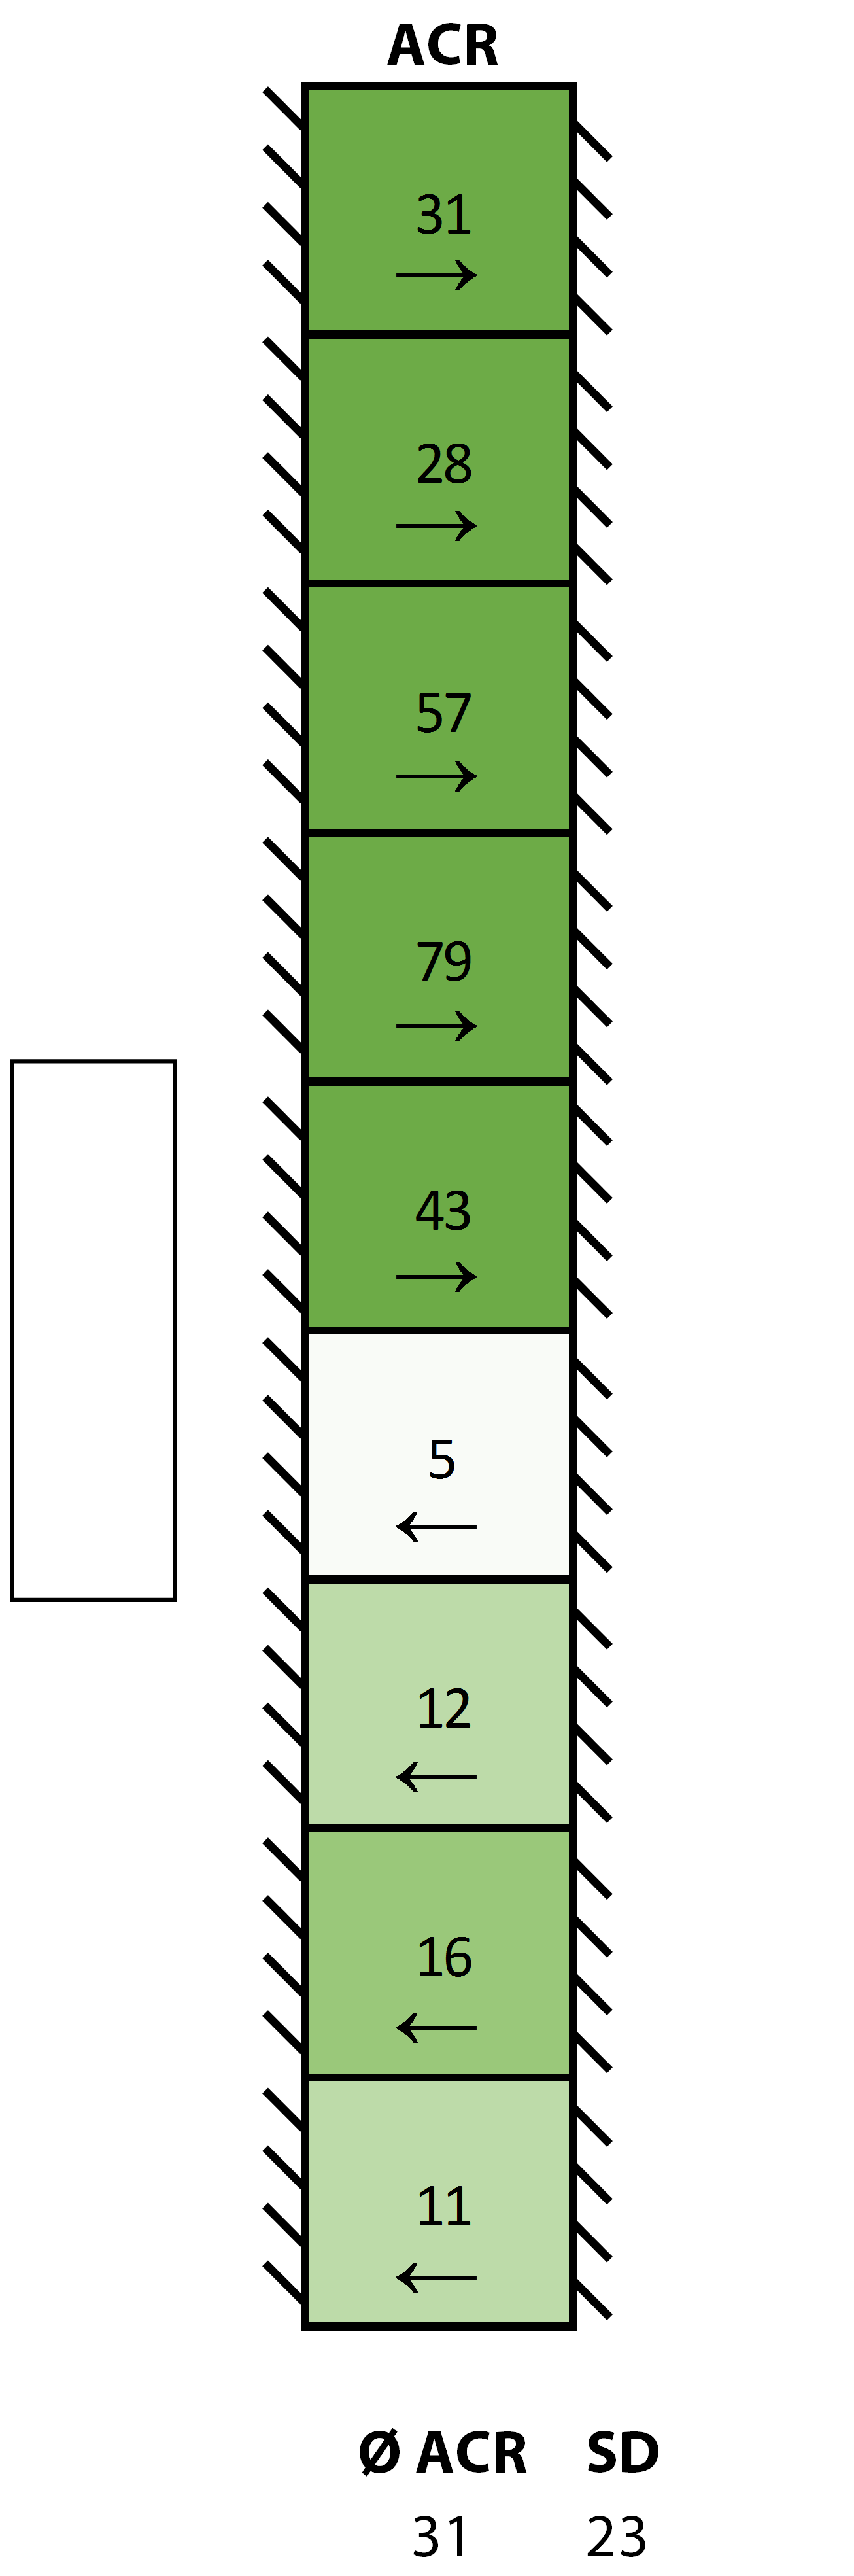
\includegraphics[width=0.14\textheight, trim= 0.00cm -2.7cm 5cm 0.45cm, clip]{images/ACR/ACR_V1-4w}}	
	\captionsetup{format=plain}
	\caption[Flow characteristics of V1-4w]{Horizontal cross-section of V1-4w depicting  $|u|$ and the flow characteristics. (\textbf{A}) Flow separation occurs in the area of the windward building block with a reattachment point of about \SI{30}{m}. (\textbf{B}) Constriction of the flow in the area of the staircase; following the continuity constraint,  the velocities increase by a factor of $\sim$\num{2}. (\textbf{C}) Local velocity differences create vortices in the windward \CR. (\textbf{D}) Indefinite flow structure in leeward \CR; the ventilation direction changed from \CR\ type (C) to type (D).}
	\label{fig:V1-4w_flow_field}	
\end{figure}
\enlargethispage*{1.0cm}



\index{BRAC!air change rates}

\blindtext[1]

\blindtext[1]


\cleartoleftpage

\subsubsection{Impact of the number of windows}
\index{BRAC!effects!number of windows}
\enlargethispage*{4cm}

\blindtext[1]


\paragraph{Air change rates}

\blindtext[1]


\paragraph{CO$_2$ concentration}

\blindtext[1]


\paragraph{Age of air}

\blindtext[1]




\begin{figure}[!htbp]
	%	\centering \hspace*{-2cm} 
	\begin{tikzpicture}[remember picture, overlay]
	\node[yshift=8cm] {
\includegraphics[scale=0.3, trim= 0cm 0cm 0cm -2cm, clip]{images/arrow_N}};
	\end{tikzpicture}
	\subfloat[][V1-4w]%
	{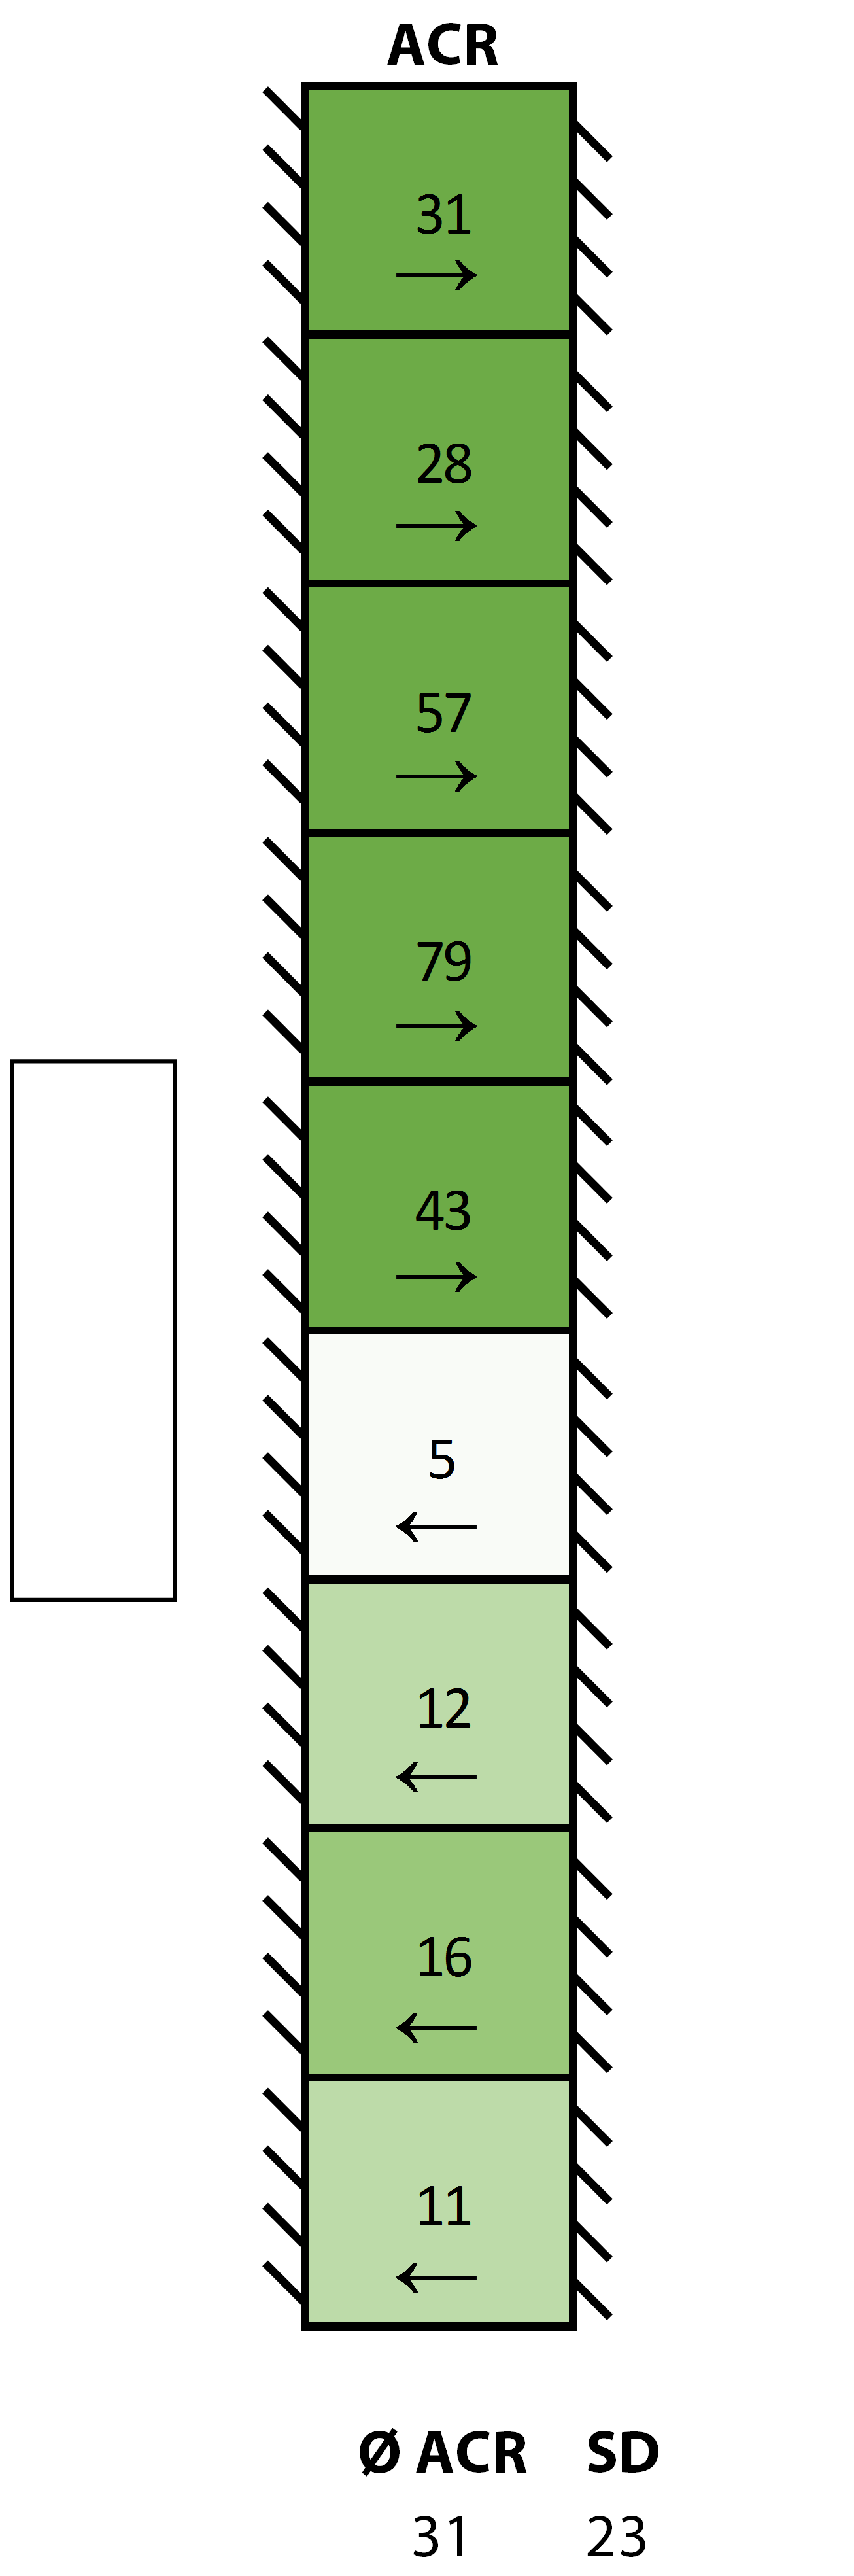
\includegraphics[width=0.135\textheight, trim= 0.00cm 0.1cm 5cm 0.45cm, clip]{images/ACR/ACR_V1-4w}\hspace*{0.5cm}
		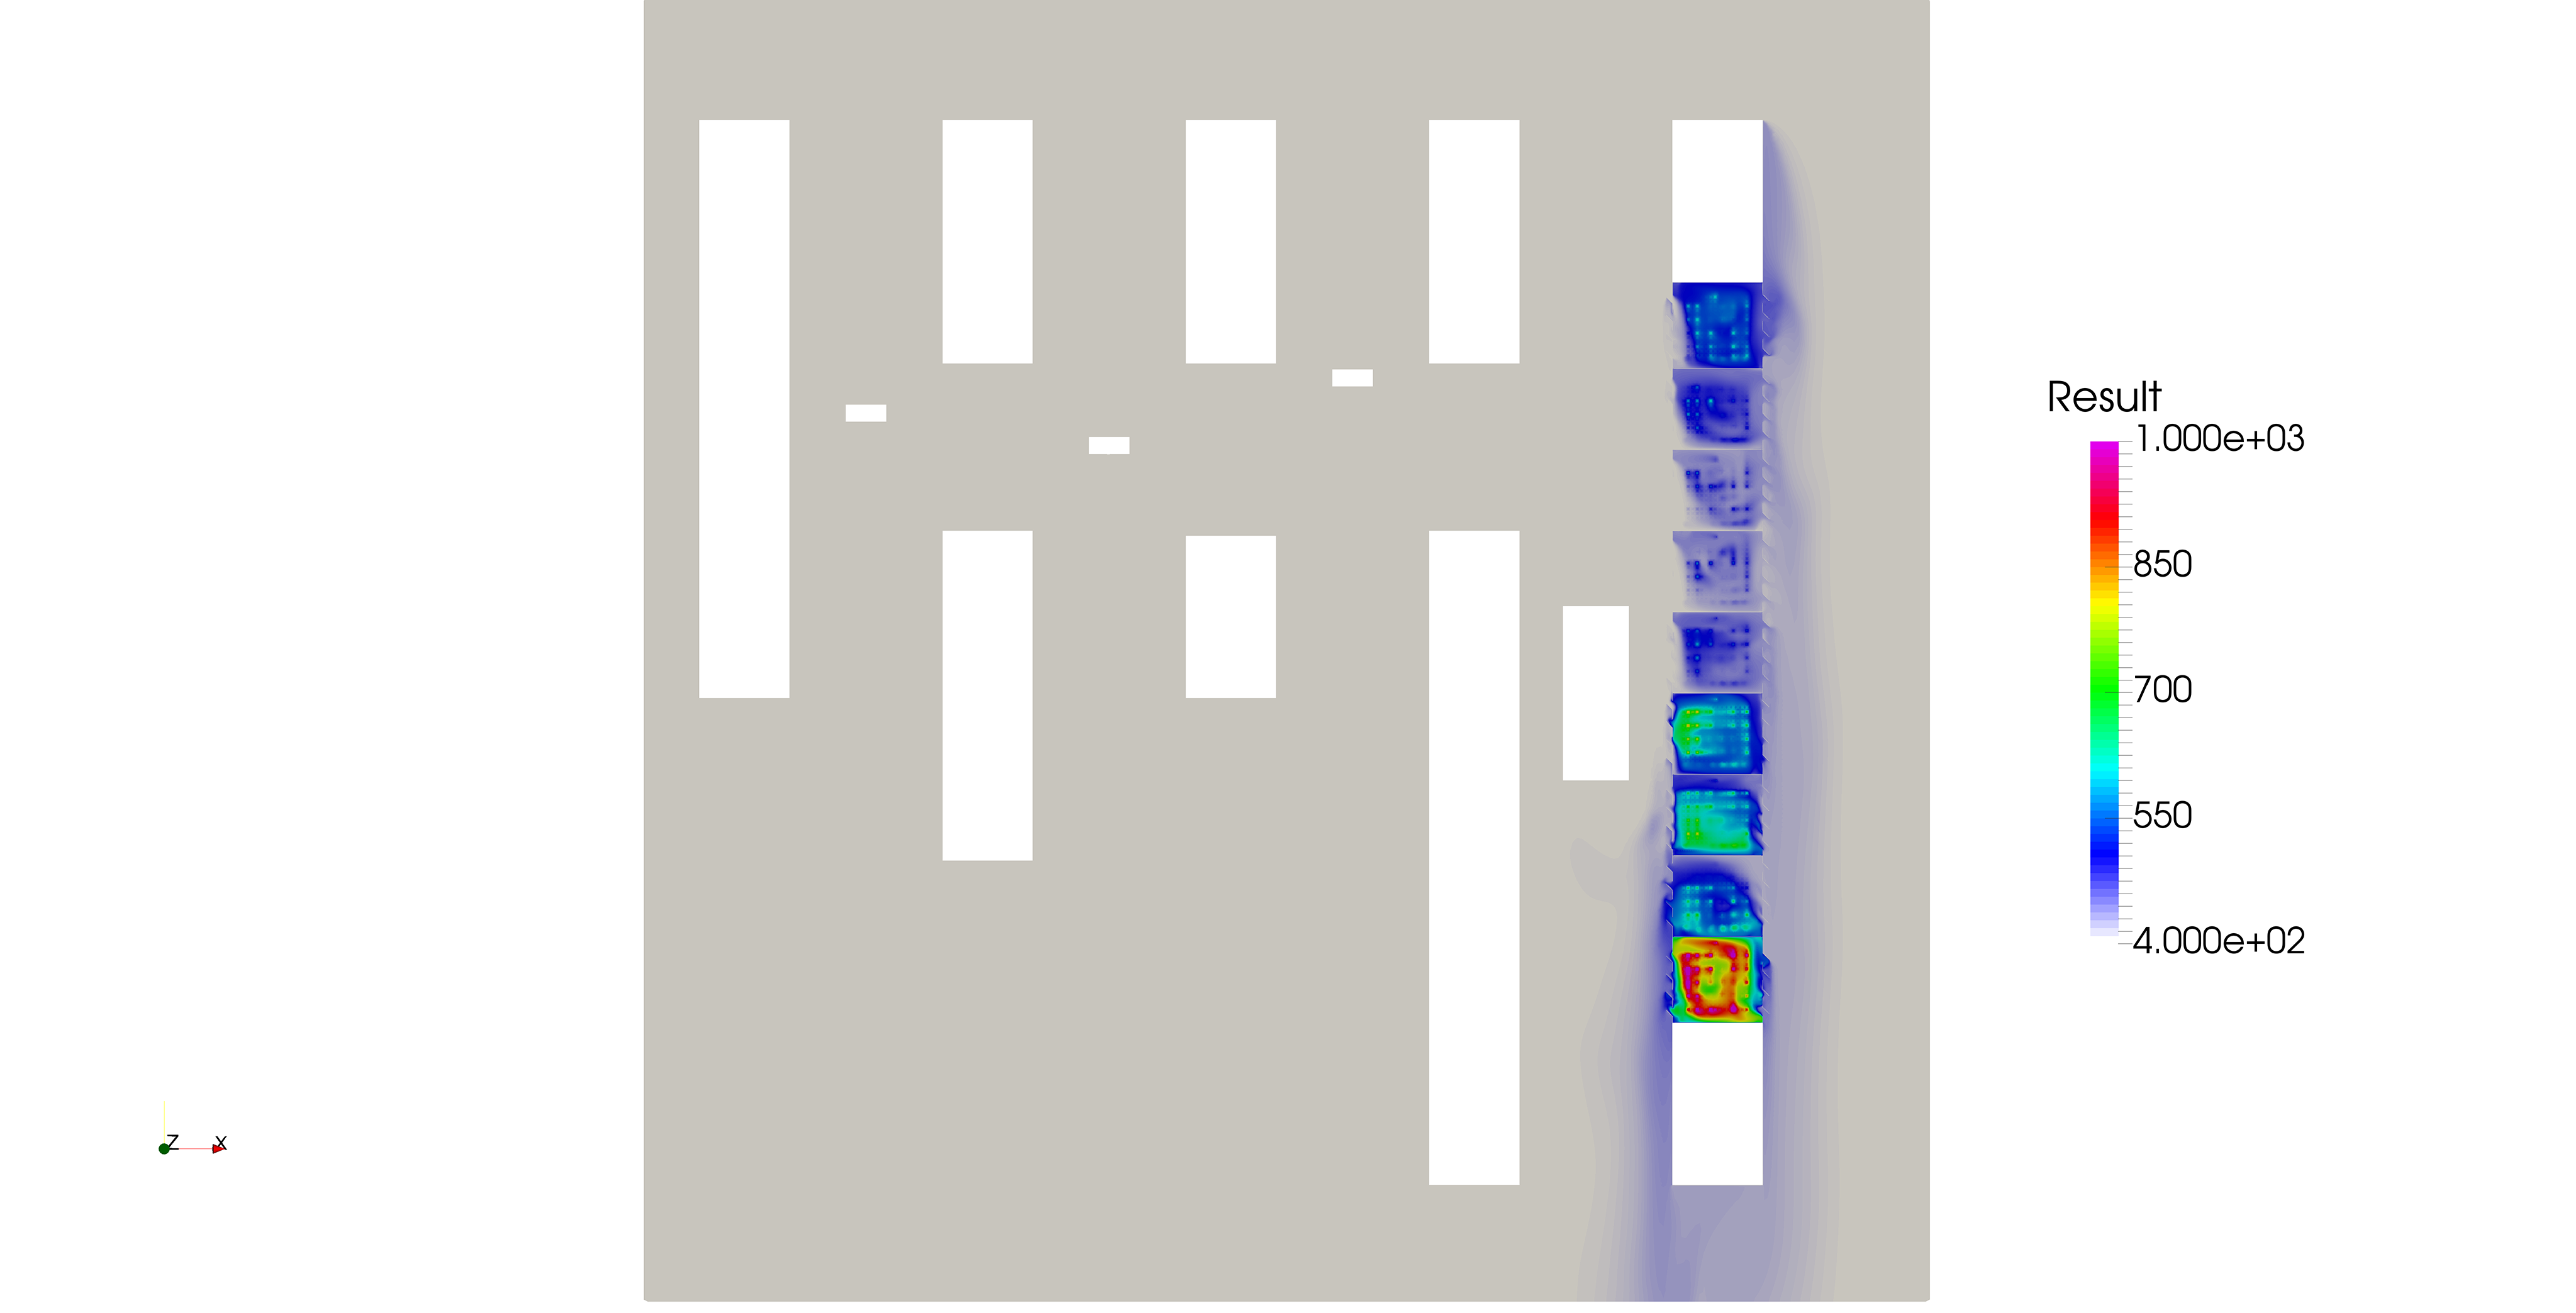
\includegraphics[width=0.162\textheight, trim= 86.5cm 11.5cm 41cm 15cm, clip]{images/CO2/V1-4w/topview_CO2}}
	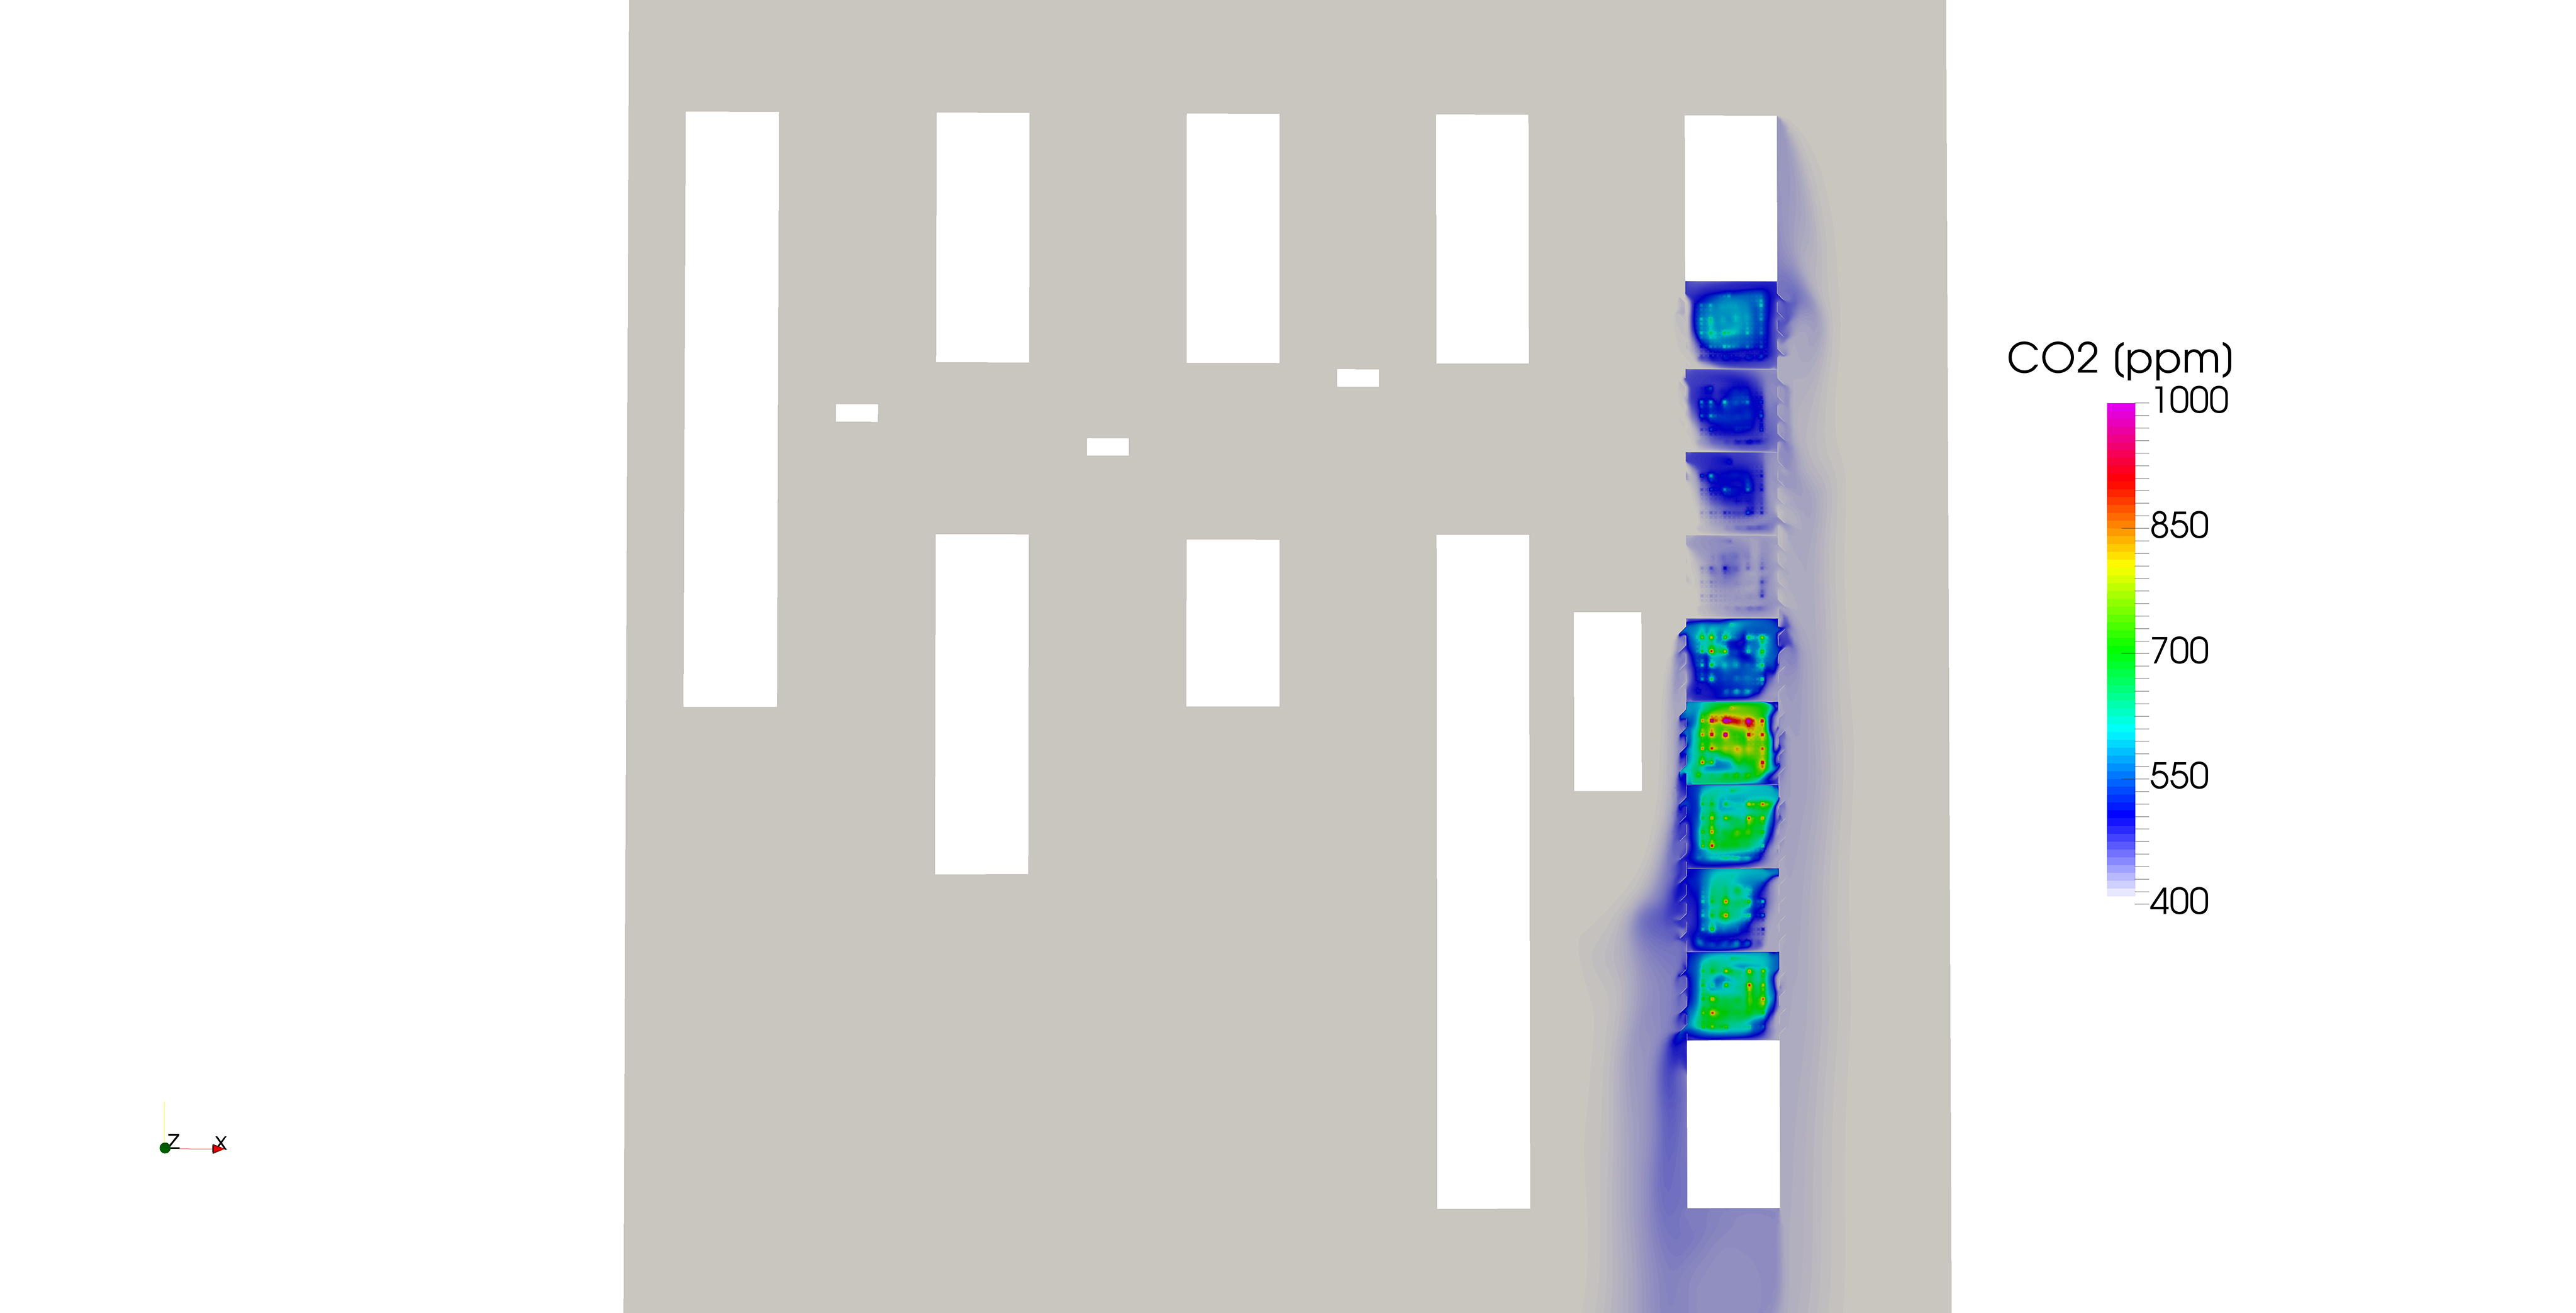
\includegraphics[width=0.09\textheight, trim= 112cm 5.85cm 19cm 10cm, clip]{images/CO2/V0/topview_CO2}\hspace*{0.5cm}
	\includegraphics[width=0.062\textheight, trim=65cm -8cm 68cm 0cm, clip ]{images/AoA/BRAC/V1-4w/topview_AoA4}
	\includegraphics[width=0.062\textheight, trim=90cm 7cm 45cm 0cm, clip ]{images/AoA/BRAC/V1-4w/topview_AoA4}  \\
	\begin{tikzpicture}[remember picture, overlay]
	\node[yshift=8cm,xshift=-3.2cm] {
\includegraphics[scale=0.3, trim= 0cm 0cm 0cm -2cm, clip]{images/arrow_N}};
	\end{tikzpicture}
		\subfloat[][\mbox{V1-1w}]		
	{\hspace*{-3.2cm}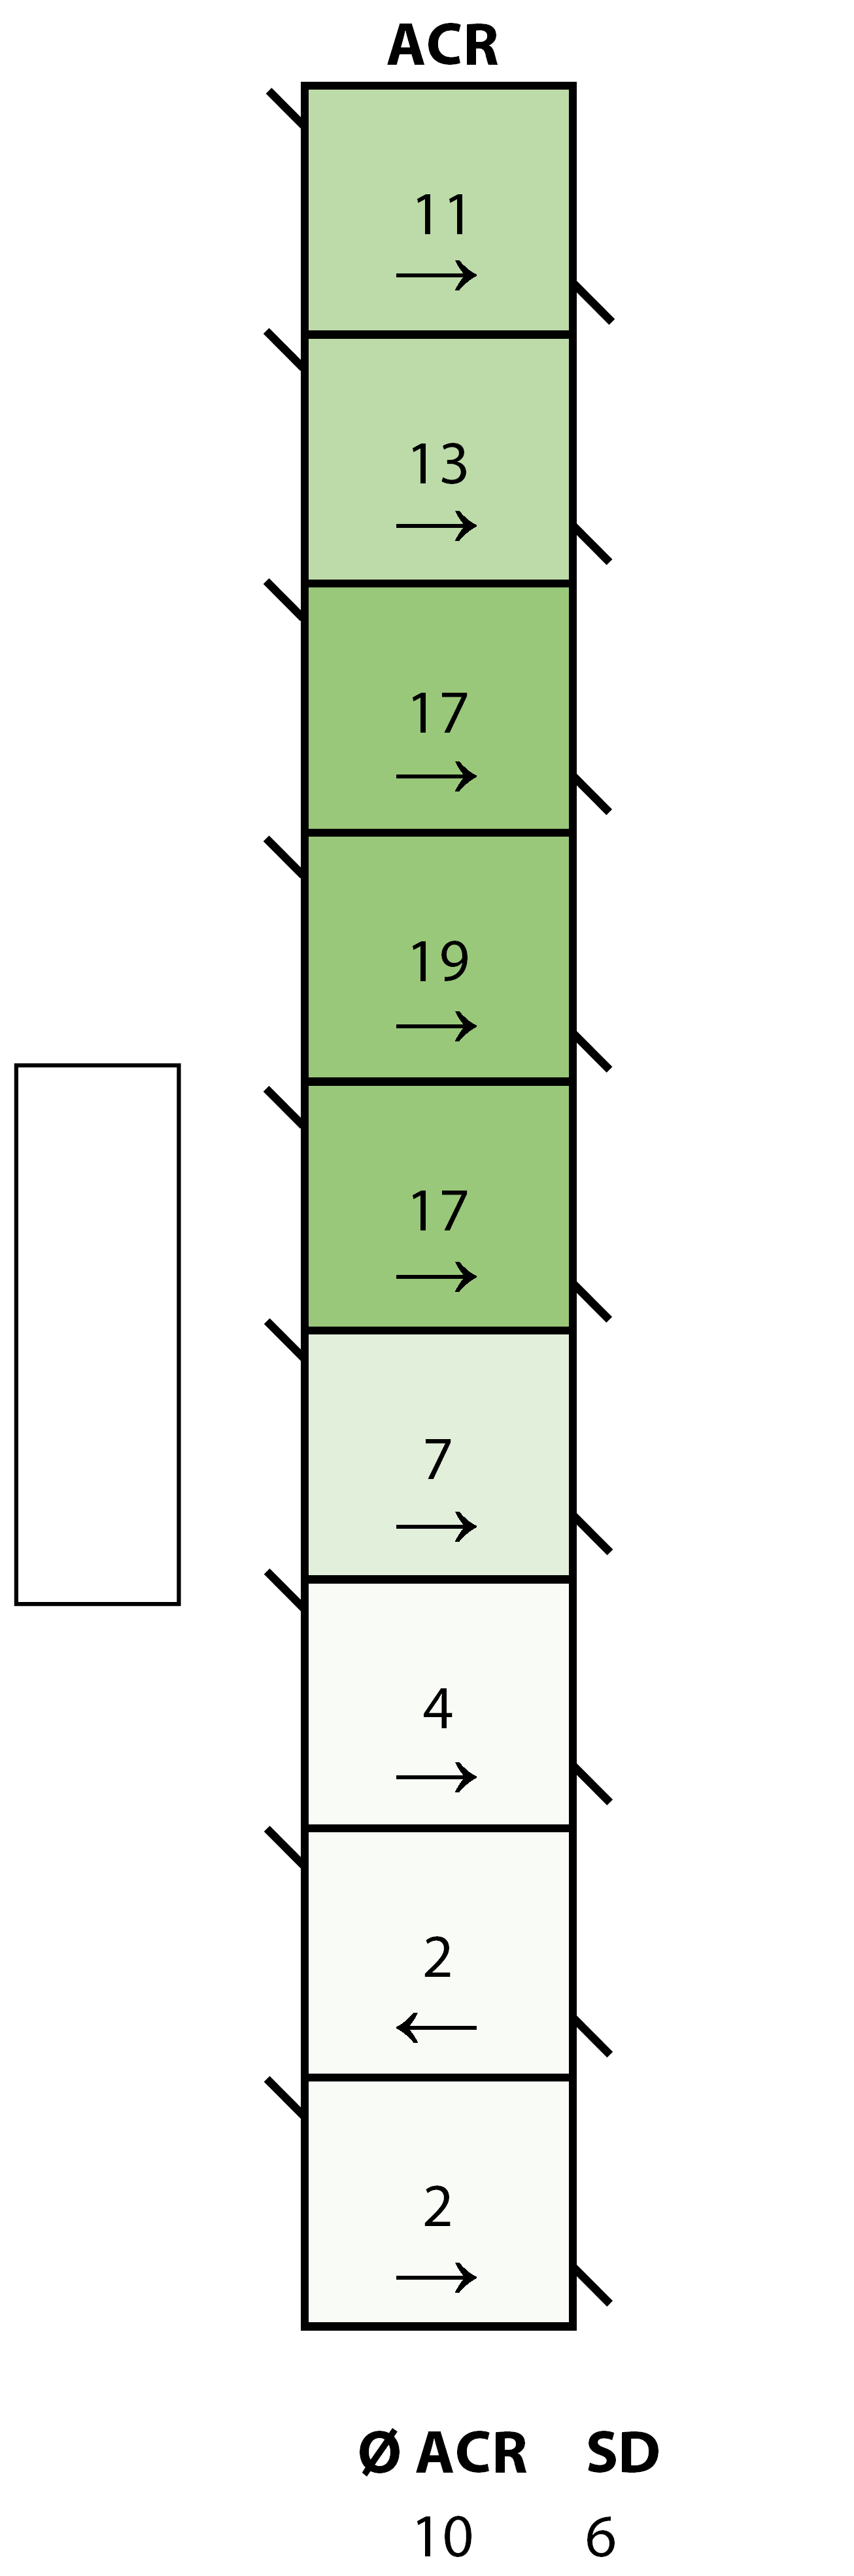
\includegraphics[width=0.135\textheight, trim= 0.00cm 0.1cm 5cm 0.45cm, clip]{images/ACR/ACR_V1-1w}}\hspace*{0.1cm}
	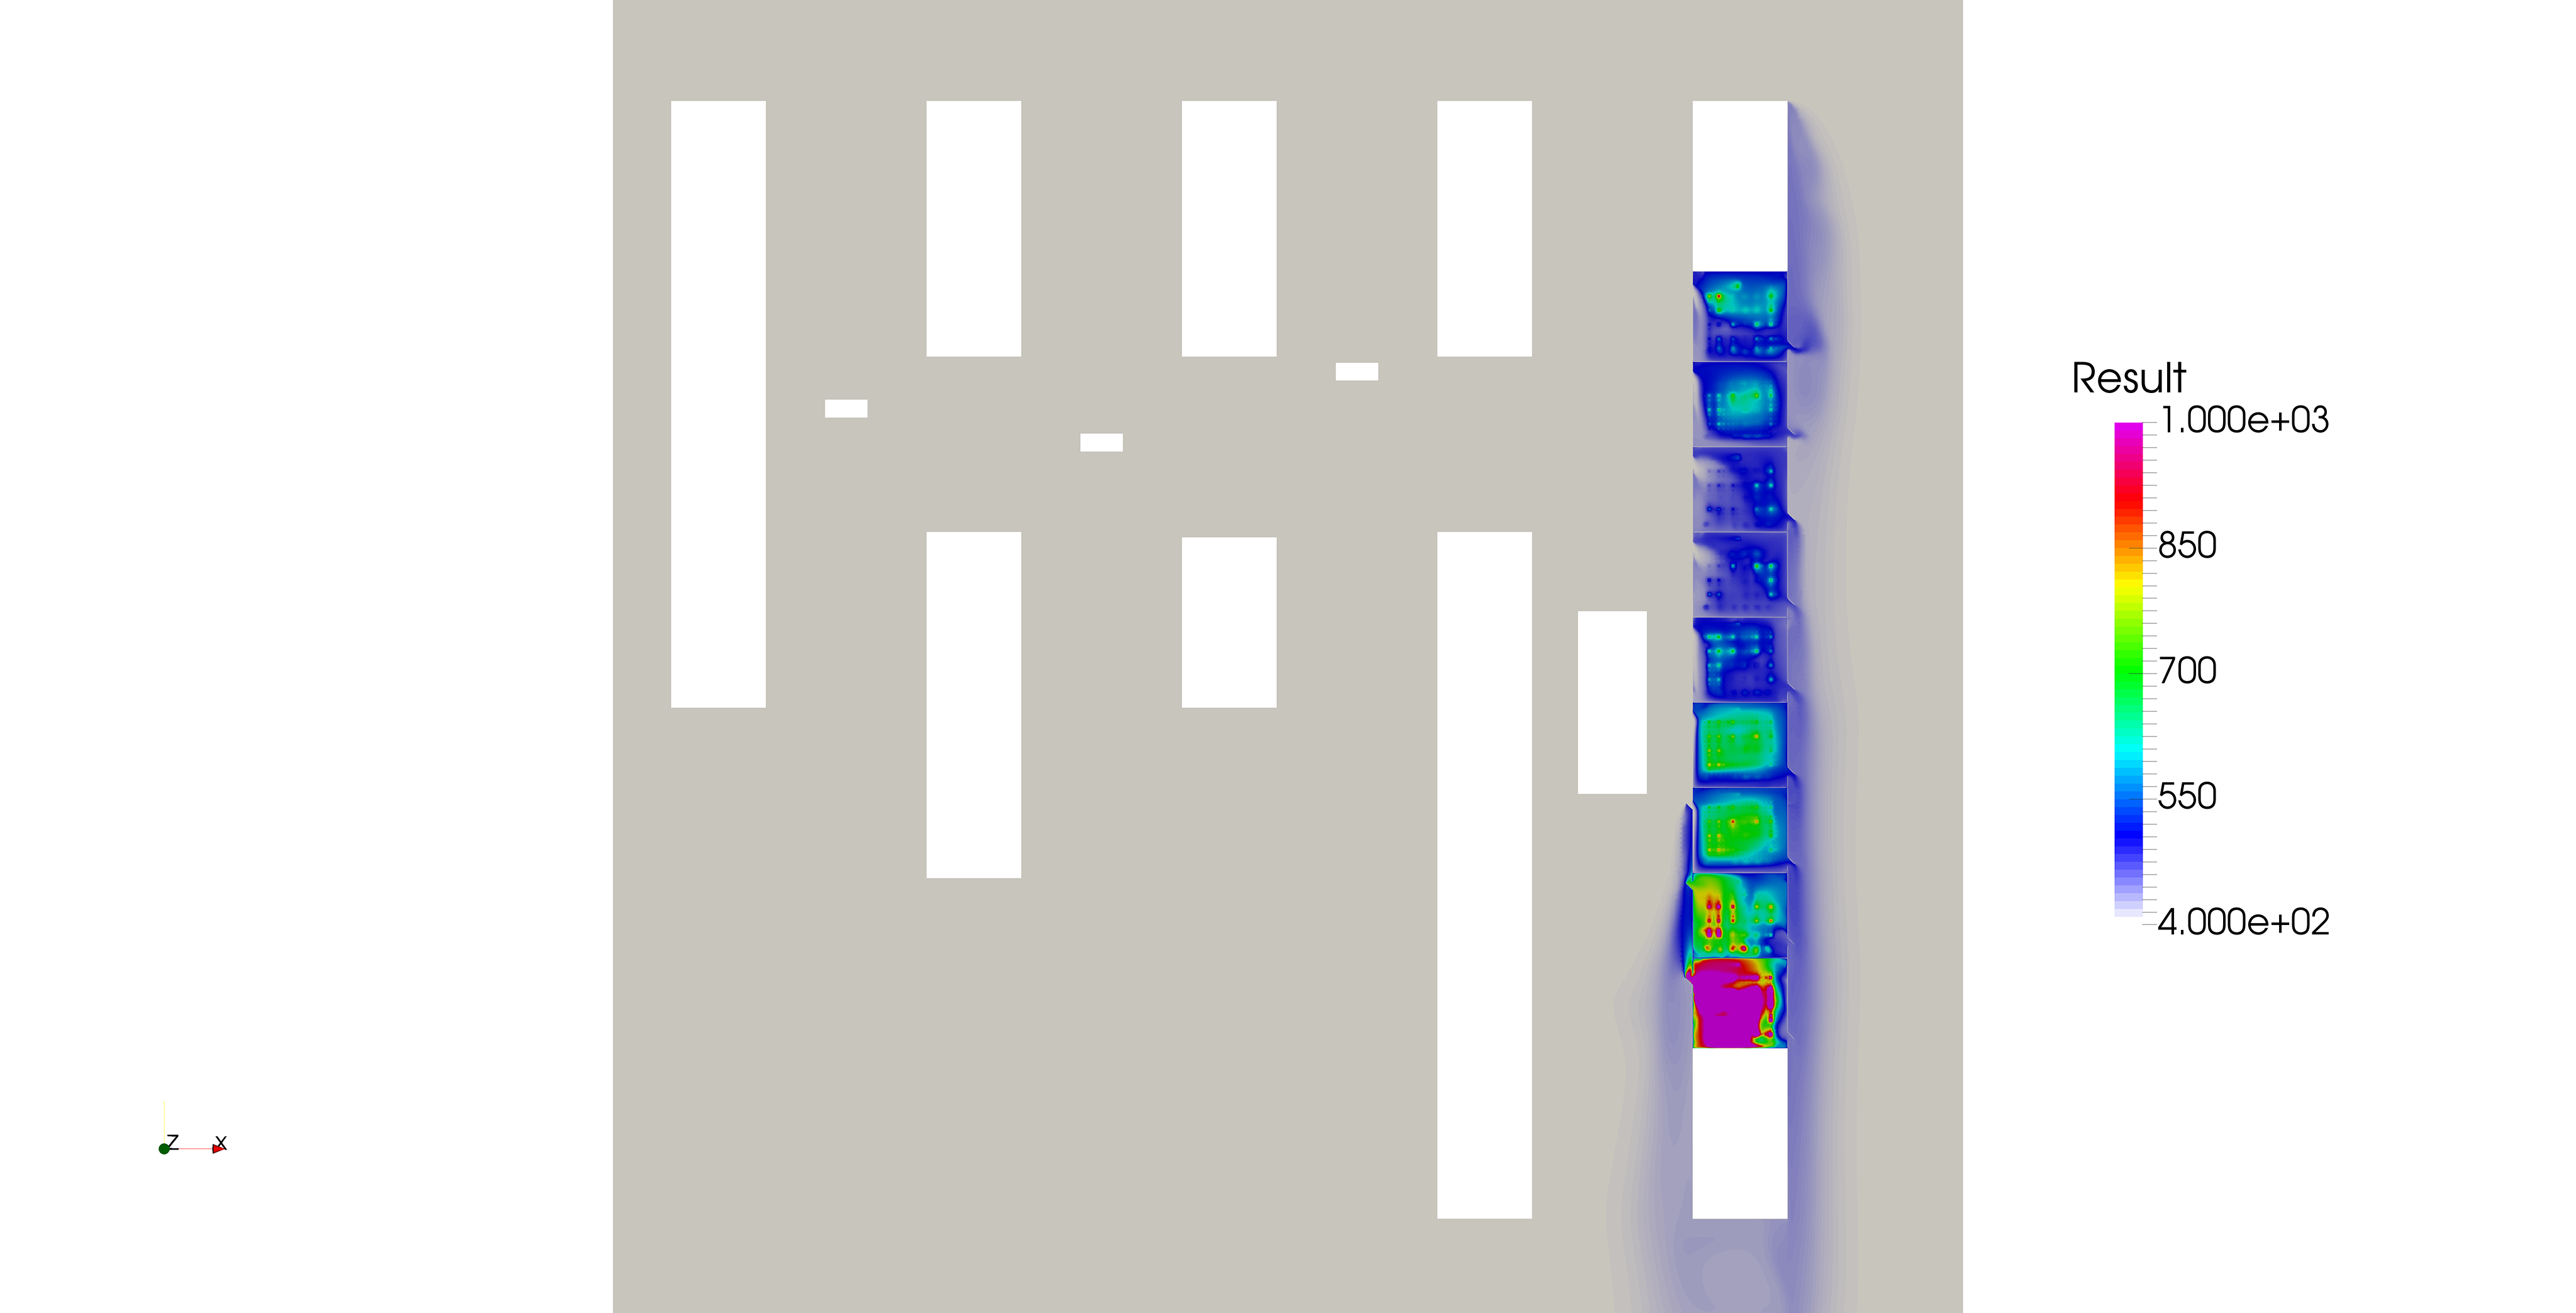
\includegraphics[width=0.160\textheight, trim= 86.5cm 11.5cm 41cm 15cm, clip]{images/CO2/V1-1w/topview_CO2}
	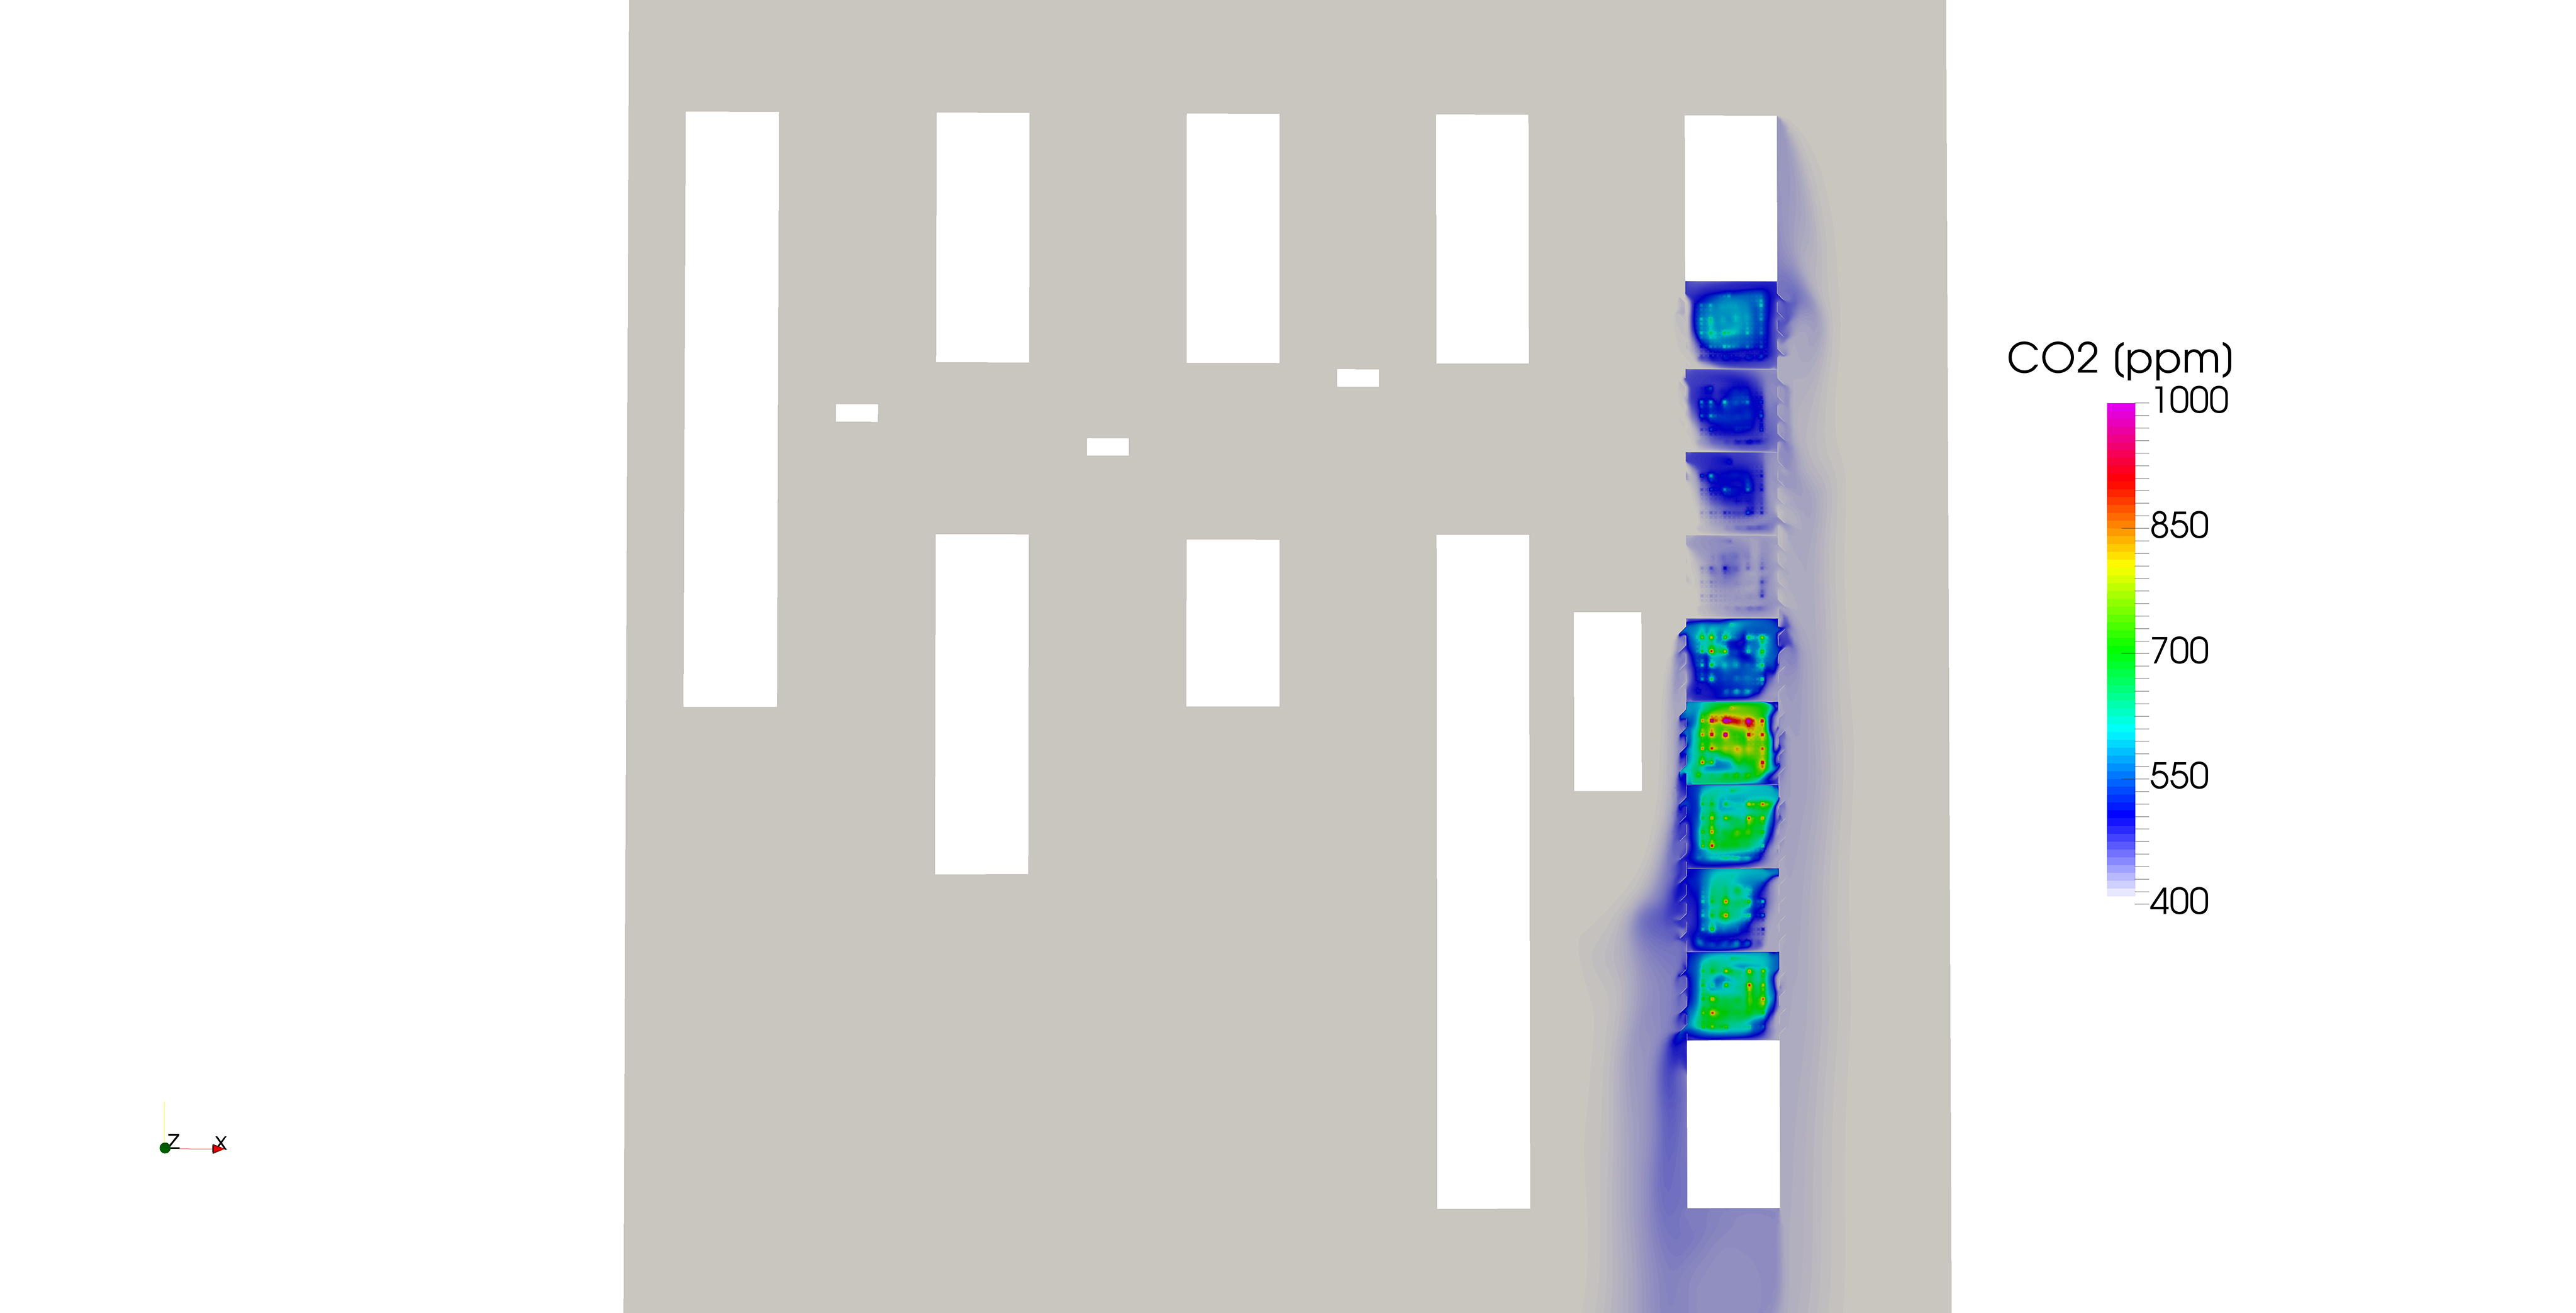
\includegraphics[width=0.09\textheight, trim= 112cm 5.85cm 19cm 10cm, clip]{images/CO2/V0/topview_CO2}
	\captionsetup{format=plain}
	\caption[Comparison of the  natural ventilation potential of V1-4w against V1-1w]{Comparison of the  natural ventilation potential of V1-4w against V1-1w. This allows us to draw conclusions how much influence the number of openings has on the natural ventilation potential.}
	\label{fig:ACR_V14w_V12w_V11w}
\end{figure}



